\section{TRABALHOS RELACIONADOS}

%Trabalhos de mineração de textos (Lucas, Priscila, morais e ambrósio)
Explorar comentários de vídeos do Youtube é uma área de pesquisa recente e ainda em crescimento. Os trabalhos de \citeonline{ammari2011filteringYt} e \citeonline{schultes2013leave} são pesquisas relativamente recentes que possuem coleta, mineração e classificação desses comentários.

O trabalho de \citeonline{ammari2011filteringYt} faz parte de um grupo maior de pesquisas, que visam elaborar um modelo de usuário que possa ser utilizado em simuladores de aprendizagem. Seu foco é apresentar uma técnica de filtragem de comentários com baixo valor semântico para o domínio selecionado, coletados de mídias sociais. A técnica proposta combina aprendizagem de máquina, mineração de dados, e análise semântica, a fim de obter comentários que sejam relevantes para o domínio desejado. A construção do modelo foi feita utilizando os classificadores Naïve Bayes Multinomial e Árvore de Decisão C4.5.

\citeonline{ammari2011filteringYt} coletou 1159 comentários de 17 vídeos do Youtube, dos quais 5 vídeos tiveram 193 comentários selecionados para o grupo de controle do modelo. A técnica apresentada e utilizada por \citeonline{ammari2011filteringYt} é mostrada na Figura \ref{fig:ammari-metodologia}:

\begin{figure}[H] %use h para forçar que a figura fique abaixo do texto
	\caption{\label{fig:ammari-metodologia} Metodologia de filtragem para comentários de baixo valor semântico do Youtube.}
	\begin{center}
	    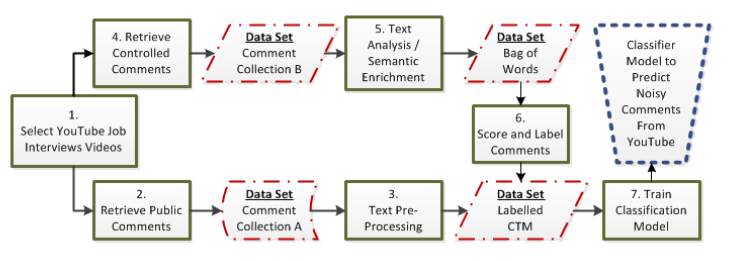
\includegraphics[scale=0.8]{figuras/figura_3.PNG} % altere o atributo scale para o tamanho da figura
	\end{center}
	\legend{Fonte: \citeonline{ammari2011filteringYt}}
\end{figure}

A metodologia da Figura \ref{fig:ammari-metodologia} consiste em:

\textbf{1.} Selecionar vídeos sobre entrevistas de emprego no Youtube.

\textbf{2.} Coletar os comentários públicos dos vídeos selecionados.

\textbf{3.} Pré-Processar os comentários obtidos.

\textbf{4.} Selecionar um grupo de comentários para grupo de controle, esses comentários são considerados relevantes para o domínio de entrevistas de emprego selecionado.

\textbf{5.} Analisar os comentários do grupo de controle, a fim de obter um Corpo de Palavras enriquecido semanticamente, relevante para o domínio.

\textbf{6.} Pontuar os comentários para facilitar sua classificação, que no caso do trabalho \cite{ammari2011filteringYt} é \textit{relevant} (relevante) ou \textit{noisy} (ruidoso - com baixo valor semântico).

\textbf{7.} Com os comentários devidamente pontuados, treinar um modelo de classificação supervisionado que irá indicar se um comentário é relevante ou não para o domínio proposto.

Os resultados apresentados por \cite{ammari2011filteringYt} indicam um alta taxa de acerto dos classificadores para os comentários obtidos e pré-processados com a metodologia proposta, sendo 86,7\% de corretude para o algoritmo C4.5 e 83,7\% para o Naïve Bayes Multinomial.

A principal diferença entre \cite{ammari2011filteringYt} e este trabalho é que apesar de focar inicialmente em vídeos com público infantil e adolescente, este trabalho é capaz de aplicar o modelo em qualquer grupo de comentários de vídeos do Youtube. Dessa forma, expandindo o domínio de aplicação. Considerando também que modelo de \cite{ammari2011filteringYt} foi testado com 17 vídeos da plataforma porém um total de 1159 comentários, este trabalho avaliou um total de 87.094 comentários pertencentes a canais difundidos entre jovens e crianças, como \textbf{Galinha Pintadinha} e \textbf{Felipe Neto}.


\citeonline{schultes2013leave} afirmam em seu texto que comentários em vídeos do Youtube são, de forma geral, mal vistos pelo público: em uma pesquisa com 95 participantes, 64\% consideram comentários do Youtube "irrelevantes", 42\% consideram agressivos e 51\% os consideram "estúpidos", sendo que somente 6\% dos entrevistados consideram os comentários em vídeos do Youtube "De essencial importância". Por outro lado, \citeonline{schultes2013leave} também afirma que 34\% dos entrevistados leem os comentários dos vídeos e que 53\% lê os primeiros três comentários antes de começar a assistir o vídeo, além de estimar um total de 96 milhões de autores de comentários ativos na plataforma, chegando a conclusão de que a seção de comentários em vídeos do Youtube é uma funcionalidade essencial e uma das mais usadas em vídeos online. Levando esses fatores antagônicos em consideração, \cite{schultes2013leave} primeiramente procura verificar se comentários em vídeos do Youtube geram algum valor agregado e como medir esse valor. \cite{schultes2013leave} também prova que através dos comentários é também possível obter uma análise semântica do vídeo em questão. 

No período de 15/03/2012 à 21/03/2012, \cite{schultes2013leave} coletou um total de 136.854 comentário dentre 304 vídeos do Youtube de categorias variadas. Para tentar descobrir se os comentários agregam algum valor para o leitor, foi proposto agregá-los em três tipos de comentários:
\begin{itemize}
    \item \textbf{Discussão:} Comentários que geram debates dentre os usuários da plataforma;
    \item \textbf{Comentários inferiores:} Comentários com ofensas ou conteúdo irrelevante para o vídeo em questão; 
   \item \textbf{Comentários substanciais:} Comentários não ofensivos que contém informação relevante e estão relacionados com o tema do vídeo em questão.
\end{itemize}
Após definir os tipos de comentários, ainda foram definidos dez subtipos a fim de tornar a classificação mais concisa. % Esses 10 tipos foram omitidos a fim de manter a brevidade desse texto.
Durante a validação do seu \textit{Dataset}, \citeonline{schultes2013leave} concluiram que "não existe um tipo de comentário dominante em vídeos do Youtube"\ e também que "30\% dos comentários são do tipo \textbf{Comentários inferiores}\", o que pode explicar a má impressão dos usuários em relação aos comentários em vídeos do Youtube.

Apesar de ter utilizado um grupo maior de comentários do que este trabalho, \citeonline{schultes2013leave}, os vídeos obtidos são de diversas categorias tornando o modelo gerado menos específico.

%Mario falcao
Sobre proteção de crianças online, \citeonline{marioFalcao2016} aborda em sua pesquisa o problema da falta de acompanhamento por parte dos pais, quanto a utilização da internet por seus filhos. 

\cite{marioFalcao2016} propos um sistema multiagente composto por agentes que coletaram e analisaram dados do Facebook. Os agentes trabalham juntos para trazer dados relevantes para o modelo de classificação, que auxilia em detectar casos de aliciamento infantil. O algoritmo utilizado para a classificação foi de árvore de decisão J48 \cite{quinlan1986induction}, implementado no WEKA, uma ferramenta de mineração de dados gratuita. O modelo foi validado com o perfil do Facebook de duas crianças, com o consentimento dos pais, e os resultados foram satisfatórios onde o modelo mostrou que uma das crianças apresentava-se em grupo de risco e estaria possivelmente sendo aliciada por adultos. 
Em comparação, o foco deste trabalho não é detectar possíveis aliciadores, mas sim determinar se a seção de comentários de um vídeo de Youtube é seguro para a criança que está assistindo o vídeo, sendo uma outra camada de proteção para as crianças. O trabalho \cite{marioFalcao2016} também chegou a verificar a eficácia do seu modelo com outros algoritmos de classificação, entre eles o Naive Bayes que é utilizado neste trabalho.

%EnyoGonçalves
\cite{EnyoGoncalves2017} estende o trabalho de \cite{marioFalcao2016}, buscando detectar automaticamente quando uma mensagem suspeita é trocada entre uma criança e um adulto. O algoritmo de classificação utilizado é Naive Bayes Multinomial \cite{metsis2006spamBayes}.

Os dados utilizados para treinar o modelo com mensagens "perigosas"\ foram coletados do site: \footnote{http://www.perverted-justice.com}. Os dados com mensagens consideradas "normais"\  foram retirados do site: \footnote{http://vircio.net}. Foram utilizadas 1610 mensagens ao todo, com um total de 9450 palavras, para as quais o Naive Bayes Multinomial obteve uma taxa de acerto de 86,33\%. Após aplicar o modelo em conversa real entre uma criança e um suspeito de aliciamento, \cite{EnyoGoncalves2017} mostrou que seu modelo é mais robusto que o de \cite{marioFalcao2016}, pois pode detectar frases de aliciadores fora de contexto e além disso, detecta frases como um todo e não somente palavras-chave.

A tabela, a seguir, apresenta uma comparação entres os trabalhos citados anteriormente e este trabalho em questão:


\begin{table}[H]
	\Caption{\label{tabela-trabalhos} Comparação entre trabalhos relacionados e este trabalho}%
	{%
		\begin{tabular}{p{4cm}p{5cm}p{6cm}} %{p{3cm}ccp{4.5cm}} não fica maior que o texto, horizontalmente
			\toprule
			Trabalho & Tipo de Aplicação &  Objetivo \\
			\midrule \midrule
    		\cite{ammari2011filteringYt} & Minerar comentários do Youtube & Filtrar comentários do Youtube com pouco valor semântico.\\
    		\hline	
			\cite{schultes2013leave} & Minerar comentários do Youtube & Verificar a relevância de comentários do Youtube.\\
			\hline
			\cite{marioFalcao2016} & Proteção de crianças online & Medir nível de exposição de crianças no Facebook.\\
			\hline
			\cite{EnyoGoncalves2017} & Proteção de crianças online & Detectar facilmente aliciadores de crianças na internet.\\
			\hline
			Este trabalho & Mineração de comentários do Youtube e proteção de crianças online & Verificar se um comentário de vídeo do Youtube é adequado ou não para crianças.\\
			\bottomrule
		\end{tabular}%
	}{%
	\Fonte{Elaborado pelo autor}
}
\end{table}


\begin{comment}
\textcolor{red}{Duas observações sobre essa tabela de comparação de trabalhos relacionados: \\
1. Prefira não deixar as colunas com valores binários. Ao invés de a coluna proteção de crianças, colocar tipo de aplicação. E como valor ao invés de sim e não descrever qual tipo de aplicação que pode ser proteção da criança.\\ <- Concluido
2. Por mais que você tenha colocado aqui as diferenças e semelhancas entre o seu trabalho e os relacionados, é necessário você descrever essa semelhanças e diferenças em algum paragrafo.} <- Checando
\end{comment}